\documentclass[t,xcolor={usenames,dvipsnames}]{beamer}

\mode<presentation>
{
\usetheme{Frankfurt}%Warsaw}
%\setbeamercovered{transparent}
%\setbeamercolor{background canvas}{bg=white}
}

% Delete these, if you do not want the table of contents to pop up at
% the beginning of each (sub)section:
%\AtBeginSubsection[]
%{
%  \begin{frame}<beamer>{Outline}
%    \tableofcontents[currentsection,currentsubsection]
%  \end{frame}
%}
%\AtBeginSection[]
%{
%  \begin{frame}<beamer>{Outline}
%    \tableofcontents[currentsection]
%  \end{frame}
%}

\usepackage[english]{babel}
\usepackage[latin1]{inputenc}
\usepackage{times}
\usepackage[T1]{fontenc}
\usepackage{verbatim}
\usepackage{url}


% Author-date citations
\usepackage[authoryear,round]{natbib}
\let\cite=\citep  % default \cite such as {\LaTeX} authors are used to

% Where \includegraphics should look for figures
\graphicspath{{figs/}}
\usepackage{epstopdf}
\DeclareGraphicsExtensions{.eps,.png,.jpg,.pdf}

\newcommand{\myhref}[2]{\href{#1}{\textcolor{Blue}{#2}}}
\newcommand{\subitem}[1]{\begin{itemize}\item #1 \end{itemize}}
\newcommand{\ghead}[1]{{\tiny #1\\}}

%%%%%%%%%%%%%%%%%%%%%%%%%%%%%%%%%%%%%%%%%%%%%%%%%%%%%%%%%%%%%%%%%%%%%%
% Title, author, logo
\title[Functional Curation]{Functional Curation}
\author{Jonathan Cooper and Gary Mirams}
\institute[Computational Biology]
{Computational Biology Group\\
 Department of Computer Science\\
 University of Oxford}
\date{8\textsuperscript{th} February 2012}

\begin{document}

\begin{frame}
\titlepage
\end{frame}
%%%%%%%%%%%%%%%%%%%%%%%%%%%%%%%%%%%%%%%%%%%%%%%%%%%%%%%%%%%%%%%%%%%%%%
\section{Functional Curation}
\subsection*{Main}

%\begin{frame}{Outline}
%\tableofcontents
%\end{frame}

\begin{frame}{What problem are we trying to solve?}
\begin{itemize}
\item Multiple models of a system are developed to explore and compare hypotheses
  \begin{itemize}
  \item How do we choose between them (for a particular study)?
  \end{itemize}
\item What functionality does a model have?
  \begin{itemize}
  \item May have to read several papers, and attempt to simulate the model
  \item This may not even be possible (at least without the author's assistance)
  \end{itemize}
\item How do we robustly parameterise models and challenge them with data?
\item When extending a model to explore a new experimental scenario, does it still reproduce the original behaviour?
\end{itemize}
\end{frame}

\begin{frame}{Models and experiments}
\begin{itemize}
\item We have languages (e.g.\ CellML, SBML) to describe mathematical models
\item Models are based on and tested by \alert{experiments}
\item We are developing
  \begin{itemize}
  \item A \alert{protocol language} to describe experiments % pre-proc, sim, post-proc, graph
  \item A tool to run these on models and compare results
  \end{itemize}
\end{itemize}
\end{frame}

\begin{frame}{Example protocols}
S1-S2 restitution
\begin{center}
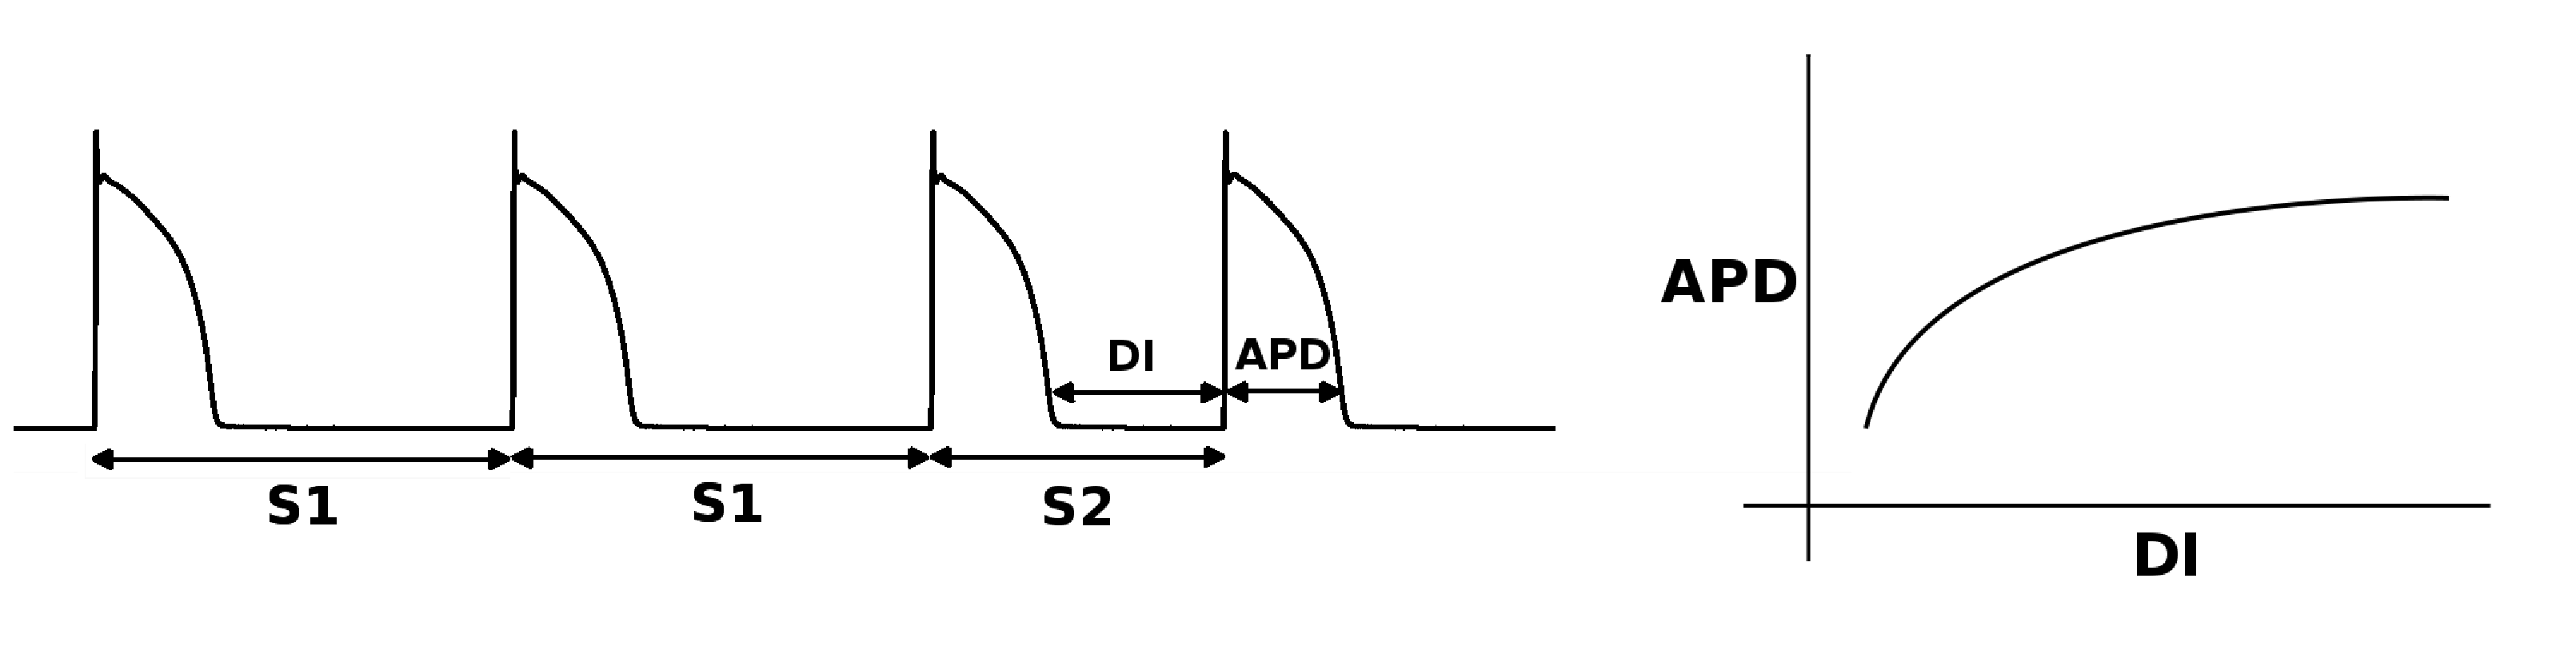
\includegraphics[width=\textwidth]{S1S2}
\end{center}
$I_{\mathrm{CaL}}$ voltage clamp
\begin{center}
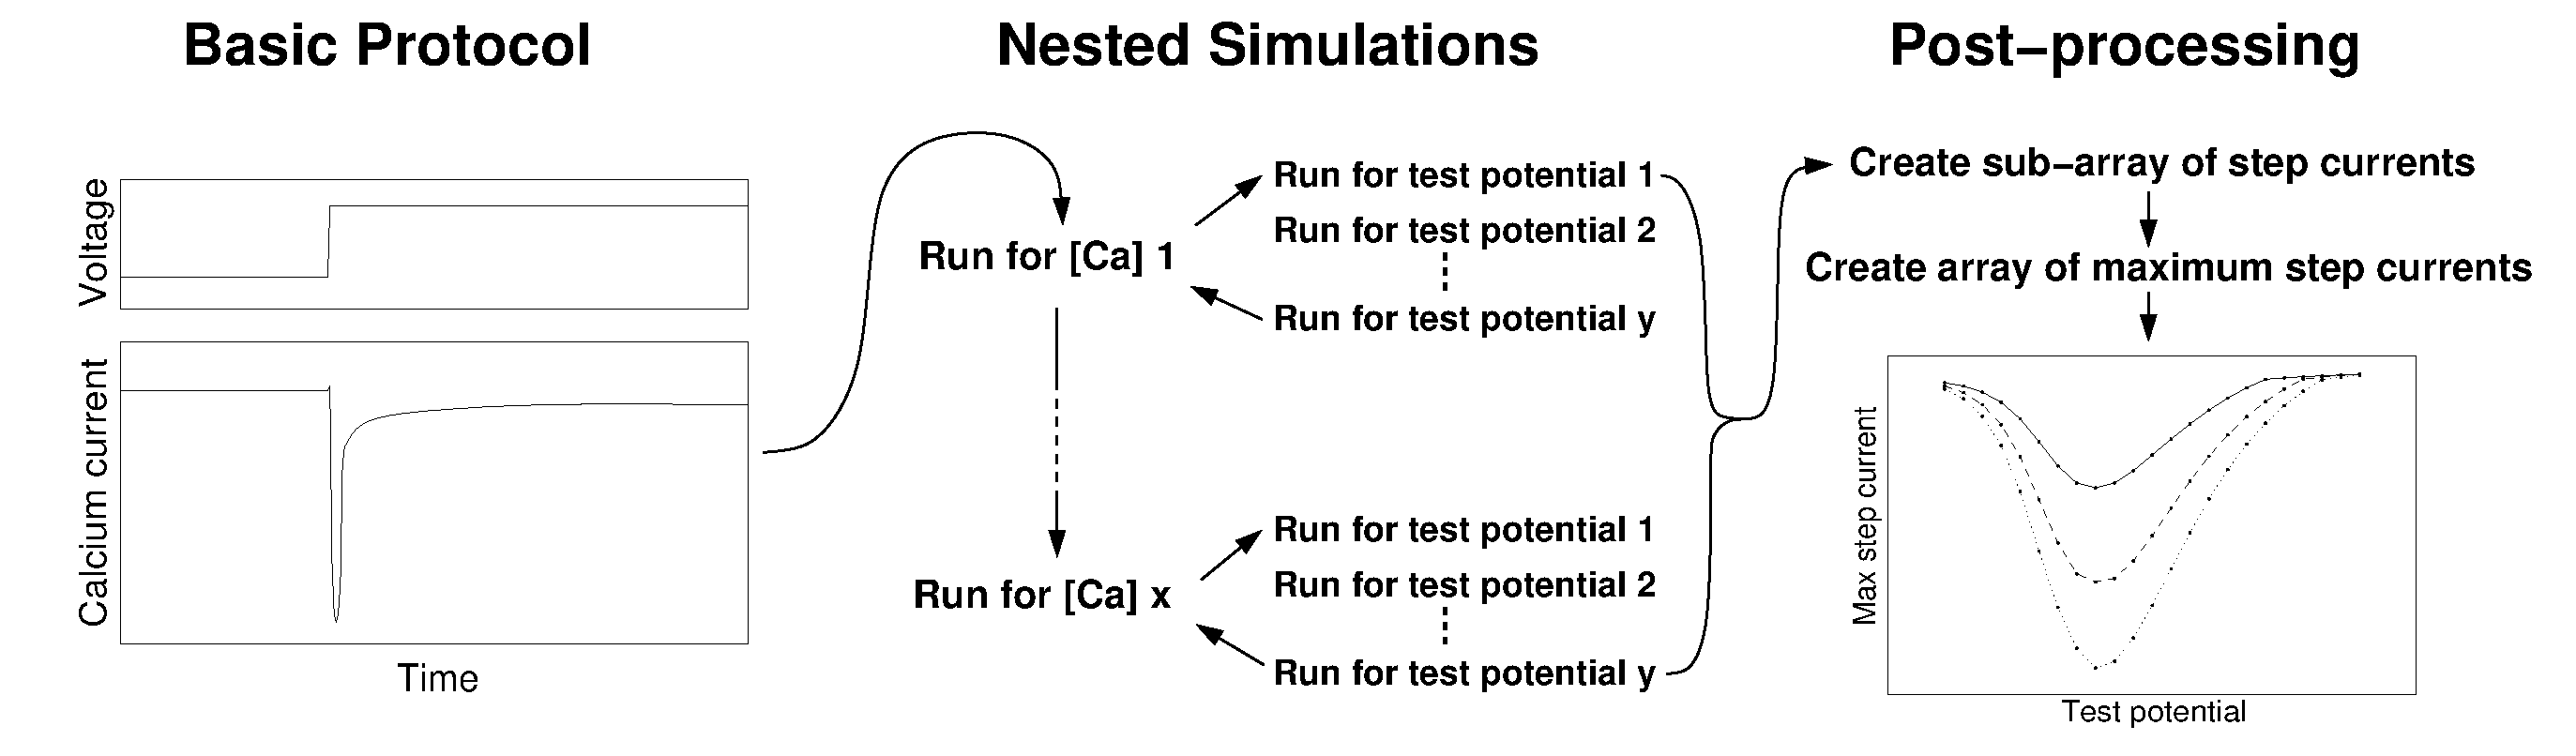
\includegraphics[width=\textwidth]{ICaLIntro}
\end{center}
\end{frame}

\begin{frame}{Example: S1-S2 restitution on canine models}
\begin{columns}[T]
\begin{column}{.33\linewidth}
\begin{center}
\includegraphics[width=\textwidth]{sicouri_dog_ventricle_s1s2_curve}\\
\vspace{.1cm}
\includegraphics[width=\textwidth]{hund_rudy_2004_s1s2_curve}
\end{center}
\end{column}
\begin{column}{.33\linewidth}
\begin{center}
\includegraphics[width=\textwidth]{winslow_model_1999_s1s2_curve}\\
\vspace{.1cm}
\includegraphics[width=\textwidth]{livshitz_rudy_2007_s1s2_curve}
\end{center}
\end{column}
\begin{column}{.33\linewidth}
\begin{center}
\includegraphics[width=\textwidth]{fox_mcharg_gilmour_2002_s1s2_curve}\\
\vspace{.1cm}
\includegraphics[width=\textwidth]{decker_2009_s1s2_curve}
\end{center}
\end{column}
\end{columns}
\end{frame}


\begin{frame}{Potential applications}
\begin{itemize}
\item Rational model selection: based on ability to produce expected results for set of protocols
  \subitem{Or motivate further development if none can}
\item Explore which model features are essential for particular behaviours
\item ``Test-driven'' model development: continual comparison to set of protocols and experimental data
  \subitem{Build up a published library thereof}
\item Parameter fitting to a set of protocols
\item Parameter sweeps, sensitivity analysis, \ldots
\item Build into a framework that stores models, protocols, and associated data
  \subitem{Publish alongside paper}
\end{itemize}
\end{frame}


\begin{frame}{Possible project areas}
\begin{itemize}
\item Extending the capabilities of the system
  \begin{itemize}
  \item Enhanced usability, in general or for a specific problem domain
  \item Performance improvements, e.g.\ targeting GPGPUs or HPC
  \item Robust comparison with experimental data, e.g.\ parameter inference, multi-factorial fitting
  \end{itemize}
\item Applying the system to modelling problems
  \begin{itemize}
  \item Cardiac electrophysiology
  \item Cell cycle
  \item Cell-based Chaste
  \item Your area of choice
  \end{itemize}
\item Feel free to make other suggestions!
\end{itemize}
\end{frame}

\end{document}
